Assembly commands also deserve their own form of abstraction, primarily in the context in which they are used. Using sorting as an example, changing a single greater-than comparator to a less-than comparator does not change the fact that the program is sorting, all it changes is the sorting order from increasing to decreasing. In order to allow for greater robustness in program types, our system must be able to take the context in which a specific command is used into account. One of the most effective methods of this is Word2Vec \cite{mikolov2013distributed}, which is able to identify terms used in similar contexts and can even be extrapolated to higher-level relationships (such as man->woman being similar to king->queen). Using the embeddings learned from Word2Vec, we gain a numerical representation of each command's context, with more similar commands sharing similar contexts. 

The small-scale experiment results of Word2Vec are shown in the T-SNE plot in Figure \ref{fig:tsne}. The findings shown in the plot correspond relatively well to human understanding, as most of the jump comparators are close to each other (jle, jg, jge); however, je is actually quite far from the rest of the comparators. We believe this is the result of the small data sample (16 documents) skewing the results. Once the high-dimensional embedding representations of terms were found, we applied hierarchical clustering to them and used our best understanding of command similarity to define the cutting point. Though this approach was adequate to confirm the validity of our system, a more formal study of assembly language usage would be preferred to validate the contexts in which commands are used and how they relate to one another. The results of this are shown in Figure \ref{fig:clust}. Both of these processes are repeated for the larger (about 850 documents) dataset, though the results of those embeddings and clusters are not shown in this paper as the images are too cluttered to be meaningfully presented.

\begin{figure}
  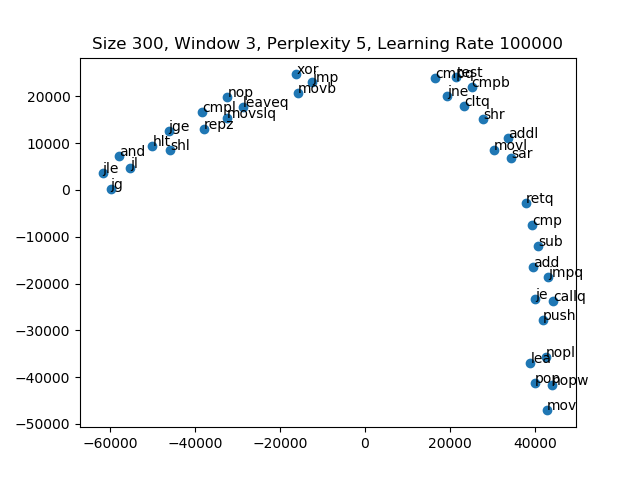
\includegraphics[width=\linewidth]{./figures/tsne_small.png}
  \caption{T-SNE plot of small-scale data Word2Vec results.}
  \label{fig:tsne}
\end{figure}

\begin{figure}
  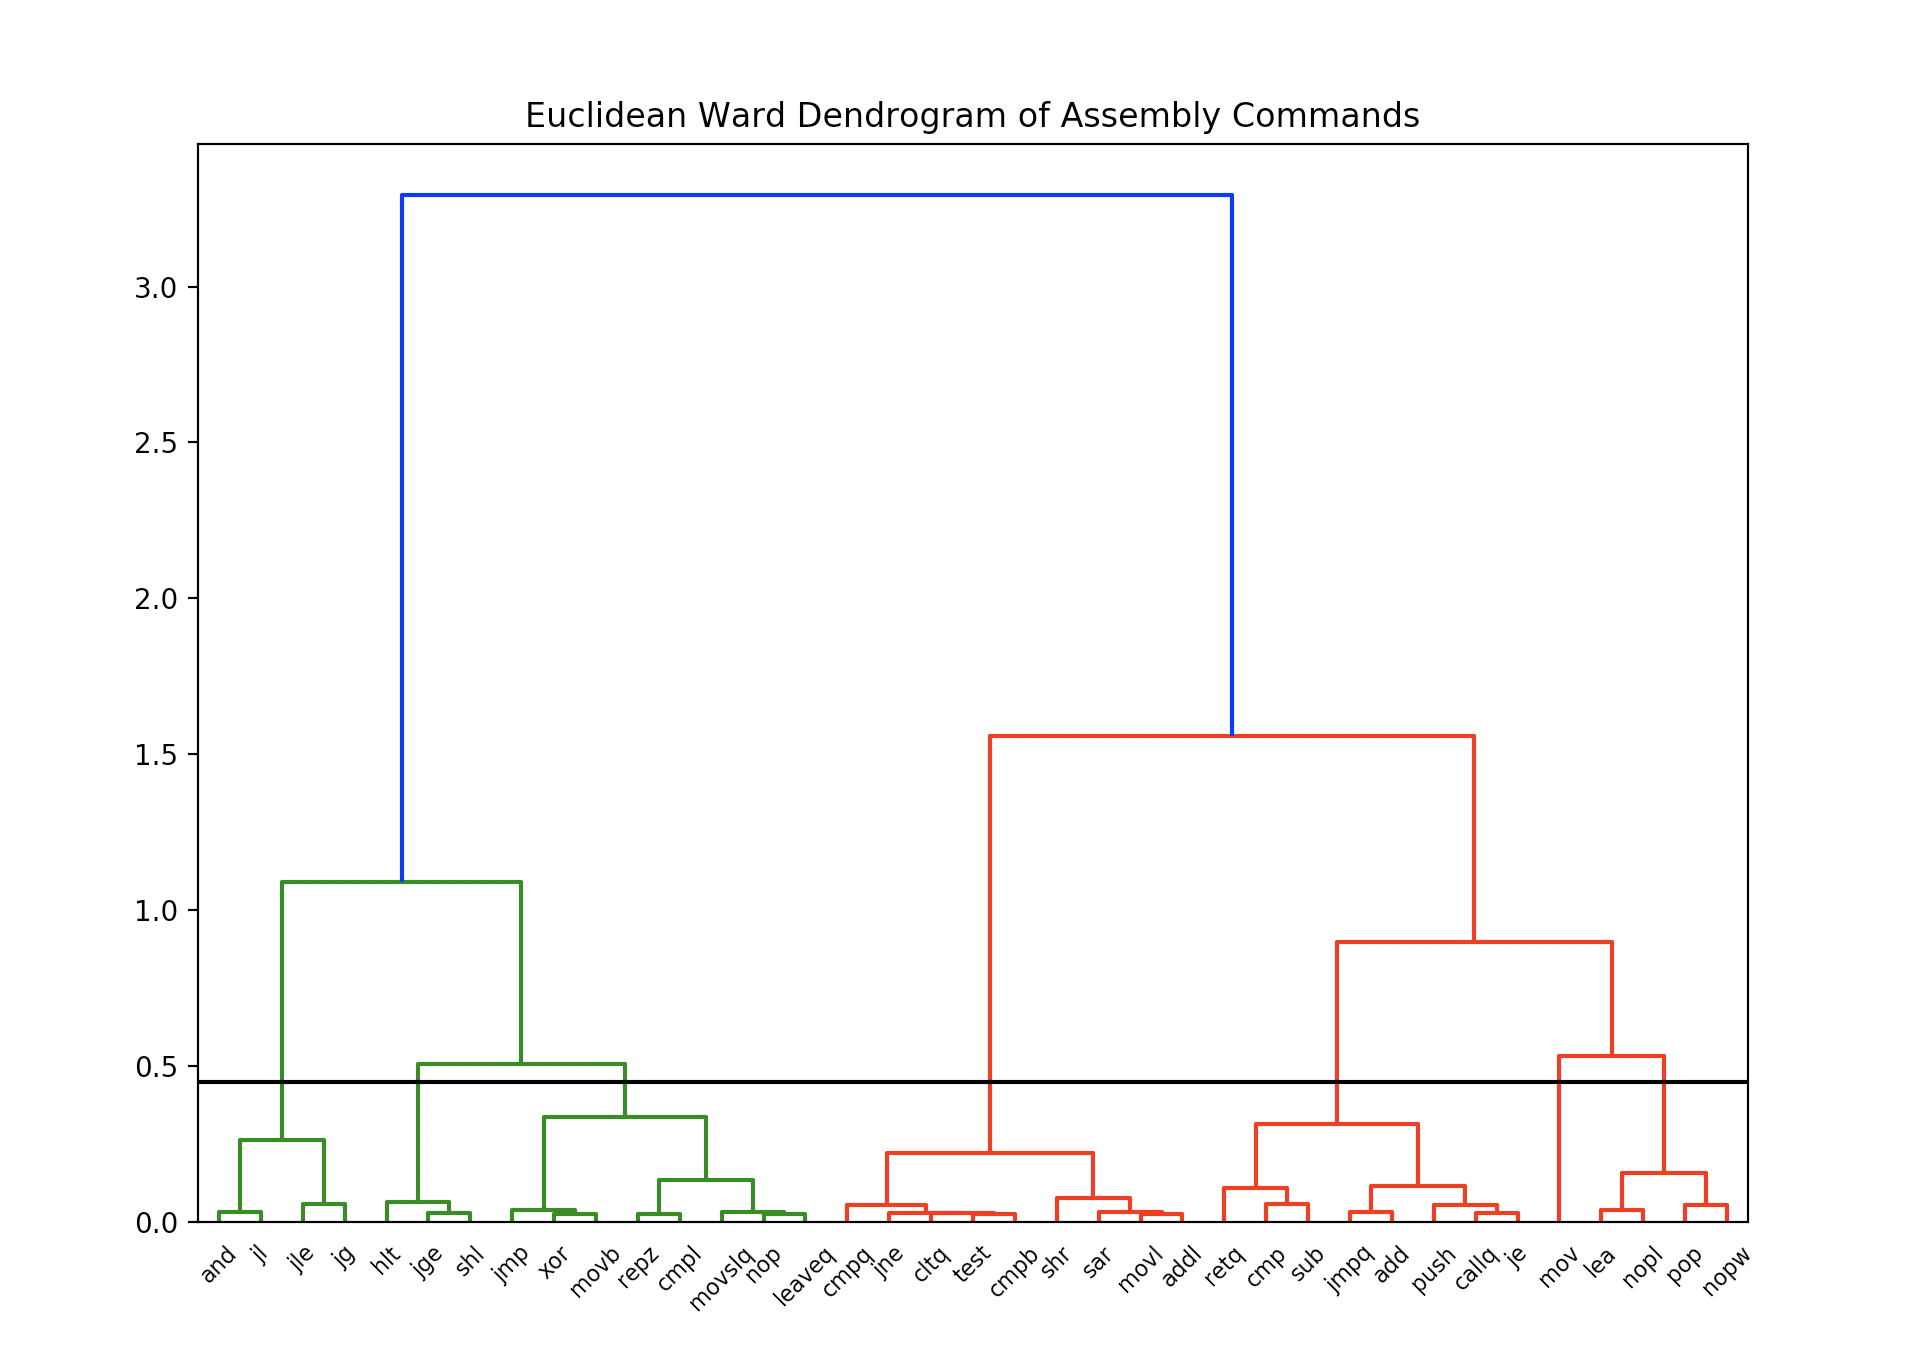
\includegraphics[width=\linewidth]{./figures/clust_small.png}
  \caption{Hierarchical Clustering results of the small dataset.}
  \label{fig:clust}
\end{figure}